\section{理论}
在本节中, 我们通过混合分布模型来说明模型的建立过程. 其中加速密度聚类算法是通过一些计算和分析给出的, 堆积速度和叠前时偏移速度模型是通过对聚类中心进行插值估计出来的. 
\subsection{混合分布模型}
\rr{同相轴局部斜率}包含地下反射的几何和速度信息. 有了估计出的\rr{同相轴局部斜率}, 我们可以用简单的一对一映射算子在时域中成像. 从反射时差的经典双曲假设开始: 

\begin{equation}
    t^2(h)=\tau_0^2+\frac{h^2}{V_{\mathrm{NMO}}^2(\tau_0)}
\end{equation}

其中$\tau_0$为双向零偏距走时, $t(h)$代表偏移量$h$处记录的双向走时, $V_{\mathrm{NMO}}(\tau_0)$为叠加速度. 我们将$t(h)$相对于$h$的导数表示为$p_h$(走时斜率):
\begin{equation}
    p_{h}(t, h)=\frac{d t}{d h}=\frac{h}{t V_{\mathrm{NMO}}^{2}\left(\tau_{0}\right)}
\end{equation}
通过上述两个方程, 叠加速度速度$V_{\mathrm{NMO}}(\tau_0)$和零偏距走时$\tau_0$可以被有效的表示出来(\cite{Ottolini1983, Fomel2007}), 如下面的两个公式所示: 
\begin{equation}
    V_{\mathrm{NMO}}\left(\tau_{0}\right)=\sqrt{\frac{h}{t p_{h}(t, h)}}
    \label{equ:3}
\end{equation}
和
\begin{equation}
    \tau_{0}=\sqrt{t^{2}-t p_{h}(t, h) h}
    \label{equ:4}
\end{equation}
为了在每个CMP道集上得到一个稳健的\rr{同相轴局部斜率}估计$p_h$, 我们采用了了PWD(\cite{Fomel2002, Chen2013})算法. 在具体应用中可以将斜率估计算法用其他算法进行替换. 域$\{t,h\}$上的单个CMP道集数据点通过方程(\ref{equ:3})和(\ref{equ:4})映射到零偏距走时和叠加速度域$\{\tau_0,V_{\mathrm{NMO}}\}$. 在偏移点的附近, \rr{同相轴局部斜率}接近零. 因此, 我们不使用零偏移点附近的数据. 与通过图像扭曲的速度图不同的是(\cite{Fomel2007}), 我们不再使用数据点的振幅. 数据点以相等的权重被映射到新的空间中. 对于实际数据的应用, 可以用从估计斜率中得到的局部相干性来分配每个要映射的数据的权重(\cite{Zhang2013}). 
\begin{figure}[htb]
    \centering
    \subfigure[使用随机噪声的人工合成 CMP 道集. \label{fig:1a}]{
        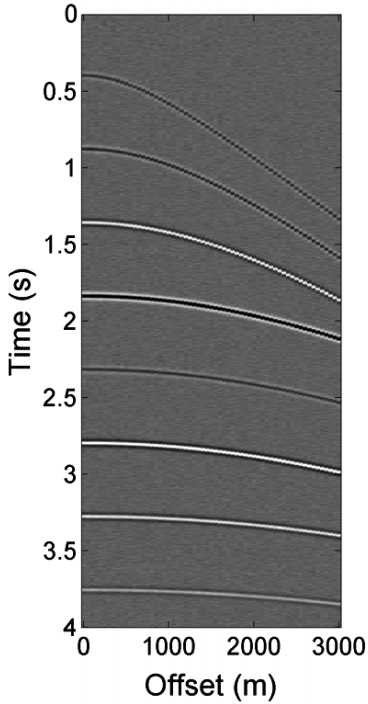
\includegraphics[scale=.2]{1a.png}
    }
    \subfigure[使用 PWD 估计斜率. \label{fig:1b}]{
        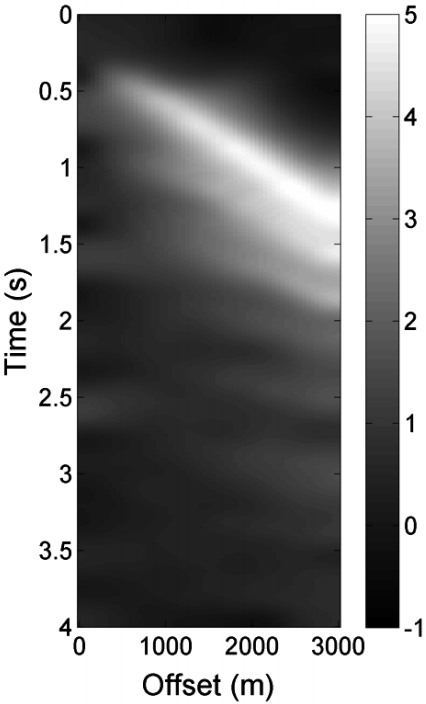
\includegraphics[scale=.2]{1b.png}
    }
    \subfigure[从局部属性映射到局部斜率的结果. \label{fig:1c}]{
        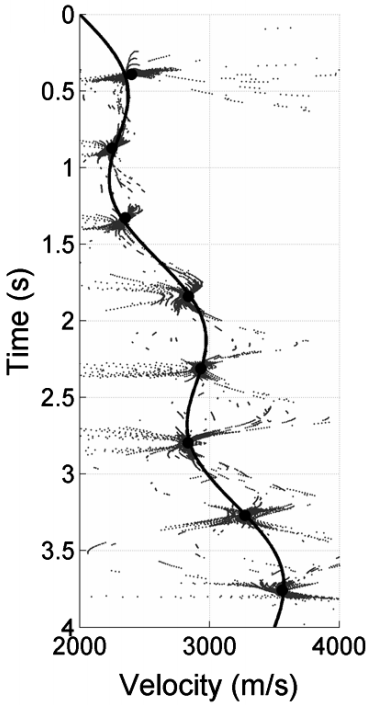
\includegraphics[scale=.2]{1c.png}
    }
    \caption{10dB随机噪声的人工数据示例. \ref{sub@fig:1c} 中, 灰色数据点是映射后的数据, 黑色圆圈是聚类中心, 黑色曲线表示真实速度. 
    }
\end{figure}
图~\ref{fig:1a} 是使用8个收集器的在速度平滑变化的介质中的简单实验. CMP道集的Ricker子波峰值频率为 20 Hz, 接收器的间隔为 50 m, 电缆总长度为 3 km, 时间间隔为4 ms, 总时间为 4 s, 该图是将速度从从 2.0 km∕s开始应用逆动校正获得的. CMP道集中添加了 10dB 的随机高斯噪声. 图~\ref{fig:1b} 描述了PWD估计出的\rr{同相轴局部斜率}. 可以看出, 估计出的\rr{同相轴局部斜率}相当平稳. 图~\ref{fig:1c} 显示了数据点映射到$\{\tau_0,V_{\mathrm{NMO}}\}$空间后的分布. 

需要注意的是, 新空间中的数据点有成簇的性质. 鉴于反射时差的双曲假设可以完全描述反射事件的运动, 并且能完美估计\rr{同相轴局部斜率}, 因此, 新空间中的数据点应该对应一次相同位置上的反射事件. 在面对实际数据时, 双曲假设不能完全描述非平面反射体, 因此, 估计出的斜率永远会有偏差, 一个反射事件会被映射成一簇. 假定双曲假设和斜率估计算法的误差遵循高斯分布, 那么, 一次反射数据的映射结果可以用一个高斯分布来表示, 其期望值为极大似然估计. 对于多与一次反射的情况, 可以直观的引入高斯混合模型. 作为高斯分布的简单线性叠加, 高斯混合模型可以表示更加复杂的密度模型(\cite{Bishop2006}). 高斯混合模型如下: 
\begin{equation}
    P(\mathbf{x})=\sum_{k=1}^{K} a_{k} N_{k}\left(\mathbf{x} \mid \mu_{k}, \sigma_{k}\right)
\end{equation}
其中, $x$为映射数据点在新空间中的位置, $N_{k}\left(\mathbf{x} \mid \mu_{k}, \sigma_{k}\right)$为高斯分布, $x$的期望为$\mu_k$, 标准差为$\sigma_k$, $K$代表单个高斯分布的总数量, $a_k$取混合系数. 分布$P(x)$是联合分布$P(x|x\in N_k)$对所有可能的状态$P(x\in N_k)$的总和, 即
\begin{equation}
    P(\mathbf{x})=\sum_{k=1}^{K} P\left(\mathbf{x} \in N_{k}\right) P\left(\mathbf{x} \mid \mathbf{x} \in N_{k}\right)
\end{equation}
其中$P(x\in N_k)$等于混合系数$a_k$. 通过寻找这$K$个聚类中心, 可以有效地计算出每个高斯分布的期望值$\mu_k$. 

在图~\ref{fig:1c} 中, 黑色圆圈代表聚类中心, 它给出了速度的极大似然解, 黑色曲线为真实的NMO速度. 可以看出, 所有的聚类中心都落在了真实的NMO速度的路径上. 聚类中心的数量为8个, 等于反射体的数量. 因此, 混合分布模型可以有效地解决计算从\rr{同相轴局部斜率}映射的速度值的极大似然解的问题. 
\begin{figure}[htb]
    \centering
    \subfigure[使用随机噪声的人工合成 CMP 道集. \label{fig:2a}]{
        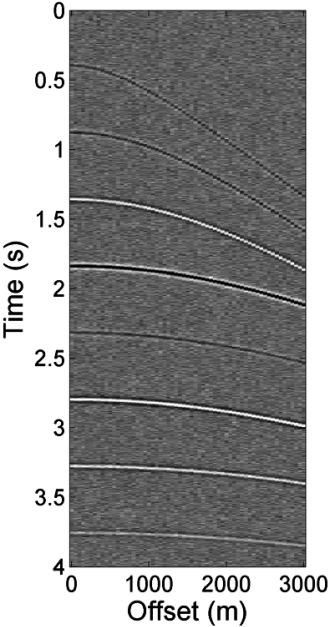
\includegraphics[scale=.2]{2a.png}
    }
    \subfigure[使用 PWD 估计斜率. \label{fig:2b}]{
        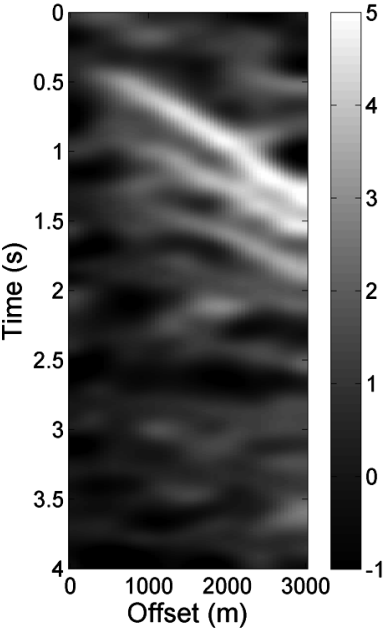
\includegraphics[scale=.2]{2b.png}
    }
    \subfigure[从局部属性映射到局部斜率的结果. \label{fig:2c}]{
        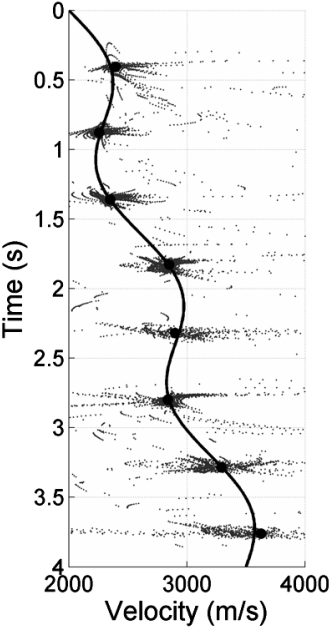
\includegraphics[scale=.2]{2c.png}
    }
    \caption{0dB随机噪声的人工数据示例. }
\end{figure}

估计出的\rr{同相轴局部斜率}的质量会因为噪声和干扰而降低. 图~\ref{fig:2a} 显示了与图~\ref{fig:1a} 中相同的CMP道集, 但添加了不同水平的随机噪声, 其信噪比为0dB. 在这种情况下, 信号的功率等于随机高斯噪声的功率. 图~\ref{fig:2b} 展示了PWD的估计出的\rr{同相轴局部斜率}. 尽管在PWD之前已经使用了带通滤波器来过滤噪声, 但估计出的\rr{同相轴局部斜率}仍受到了强噪声的影响. 图~\ref{fig:2c} 显示了在$\{\tau_0,V_{\mathrm{NMO}}\}$空间中的映射数据点, 直接映射算子给出了被高频振荡污染的部分. 在图~\ref{fig:2c} 中, 黑色圆圈代表聚类中心, 黑色实心曲线是真实的NMO速度. 可以看出, 此时所有的聚类中心仍然与真实NMO速度的路径相吻合, 这证实了聚类中心对\rr{同相轴局部斜率}的估计是稳健的. 
\subsection{加速密度聚类}
在所有用于寻找聚类中心的算法中, k-means可能是应用最广泛的那一个. 为了实施k-means算法, 需要提前知道聚类中心的数量, 但这一先验信息通常难以确定(\cite{Hamerly2004}). (\cite{Wang2012})实现了层次聚类和划分, 以便在储层表征中找到正确的聚类中心数量. 通过带分割和合并的k-means方法(\cite{Muhr2009}), 可以在合理的运行时间内选取出准确的聚类中心数量. (\cite{Lu2014})应用类似的策略来确定浅水中的衍射地震噪声. 在k-means中, 数据点总是被分配到距离最近的中心. 虽然可以用各种距离将其拓展, 但k-means还是几乎不能检测到非球形簇. 

密度聚类(\cite{Rodriguez2014})则更容易应对更一般的数据分布情况. 聚类簇数也更容易确定. 聚类中心被描述为为密度相对高于相邻点, 而且与其他密度较大的中心点距离较大的点. 对于每个数据点$i$, 其局部密度$\rho_i$和其与密度较高的点的最小距离$\sigma_i$是密度聚类中的两个十分重要的参数. 简单的$\rho_i$定义为:
\begin{equation}
    \rho_{i}=\sum_{j} \lambda\left(d_{i j}-d_{c}\right)
\end{equation}
其中, $d_{ij}$为数据点$i$与数据点$j$之间的距离, $d_c$为截止距离, 如果$d_{ij}-d_c<0$, 则$λ = 1$, 否则$λ = 0$. 该算法仅对不同数据点的$\rho_i$敏感, 这意味着其结果对参数于$d_c$是稳健的(\cite{Rodriguez2014}). 而一个数据点到密度较高的点的最小距离$\sigma_i$为: 
\begin{equation}
    \delta_{i}=\min _{j: \rho_{j}>\rho_{i}}\left(d_{i j}\right)
\end{equation}

对于密度最大的点, $\sigma_i$取值为$\max_j(d_{ij})$. 根据$\sigma_i$的定义, 我们可以得出$\sigma_i$只有在全局或局部最大值时才相对较大的. 然后选取局部密度$\rho_i$相对较大、最小距离$\sigma_i$相对较大的点作为聚类中心. 在实际应用中, 我们可以通过$\beta$的快速变化来确定中心, 即$\beta$是$\rho$和$\sigma$的乘积. 确定聚类中心后, 按照局部密度最高到最低的顺序对数据点进行分配. 数据点总是被分配到离其最近的局部密度较高的那一类中. 总的来说, 密度聚类对$N$个数据点的计算复杂度为$O(N^2)$, 详细复杂度分析见附录~\ref{Appendix:A}. 即使对于单个CMP道集, 在典型的1000个时间样本和100个源-接收器对的情况下, 也可能有105个数据点. 这使得密度聚类算法在实际数据应用也不太合适. 

在模式识别中, 输入数据空间中的几何体可能是高度折叠、弯曲或扭曲的. 瑞士卷数据集(\cite{Tenenbaum2000})就是这样一类非线性流形. 在大多数地震数据中, 数据点呈现出的结构都是线性的. 因此, 可以用高斯或类似高斯来逼近数据点的分布. 我们提出了一种基于直方图函数的加速密度聚类算法. 在统计学中, 直方图是数据分布的一种表示. 在密度聚类中所需要的局部密度由直方图函数来近似. 我们应用二维直方图分析方法(\cite{Gonzalez2002,Zhang2015})对映射后的零偏距时间和叠加速度进行分析, 得到局部密度的估计. 
\begin{equation}
    \rho=H(l_1,l_2)=m(l_1,l_2)
\end{equation}
其中, $l_1$和$l_2$分别代表零偏距时间和叠加速度, $H(l_1,l_2)$是二维直方图函数, $m(l_1,l_2)$是共同在某个组距内的零偏距时间和叠加速度映射后得到的同相轴局部斜率的数目, 这个组距用$l_1,l_2$所代表. 直方图可以用估计出的同相轴局部斜率的相干性来加权, 以保证稳健性, 因为相干性是映射属性可靠性的自然度量. 
\begin{figure}[htb]
    \centering
    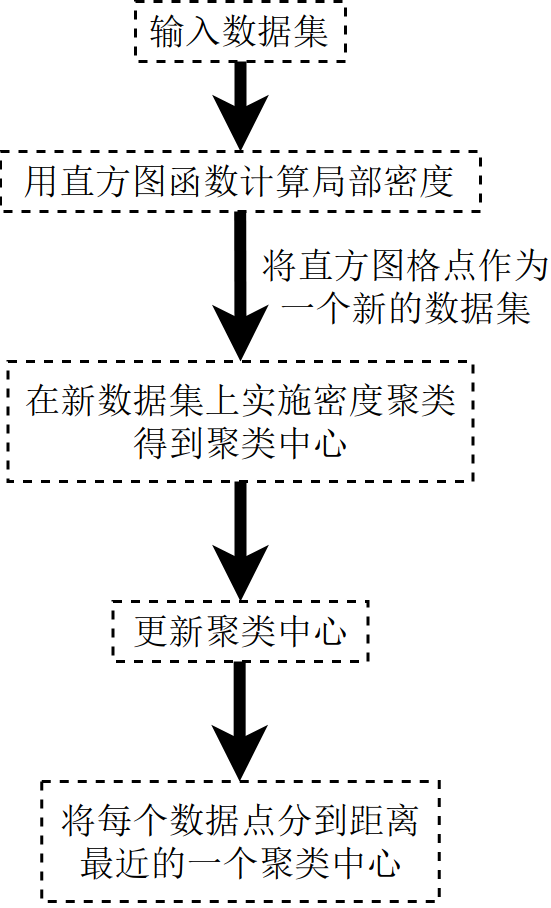
\includegraphics[scale=.18]{3.png}
    \caption{加速密度聚类算法流程图. \label{fig:3}}
\end{figure}

加速密度聚类算法的流程图如图~\ref{fig:3} 所示. 为了证明加速密度算法的性能, 我们将其应用于``S"数据集(\cite{Fraenti2006}), 
\begin{figure}[htb]
    \centering
    \subfigure[``S"型数据集. \label{fig:4a}]{
        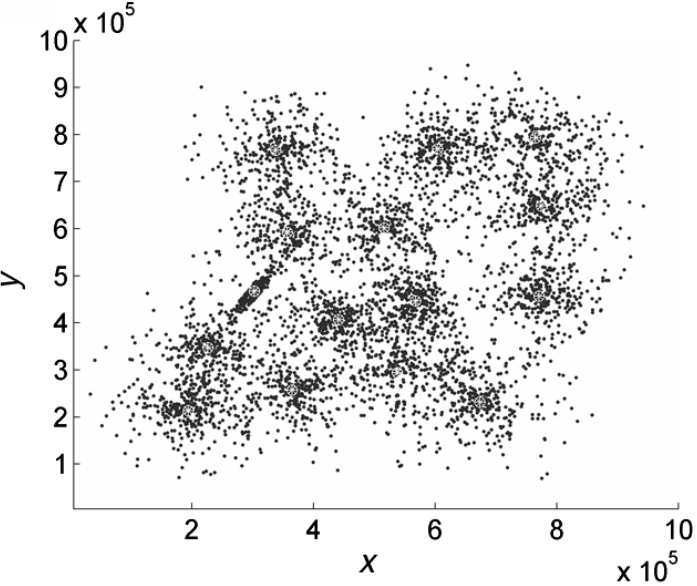
\includegraphics[scale=.15]{4a.png}
    }
    \subfigure[由直方图函数计算出的局部密度. \label{fig:4b}]{
        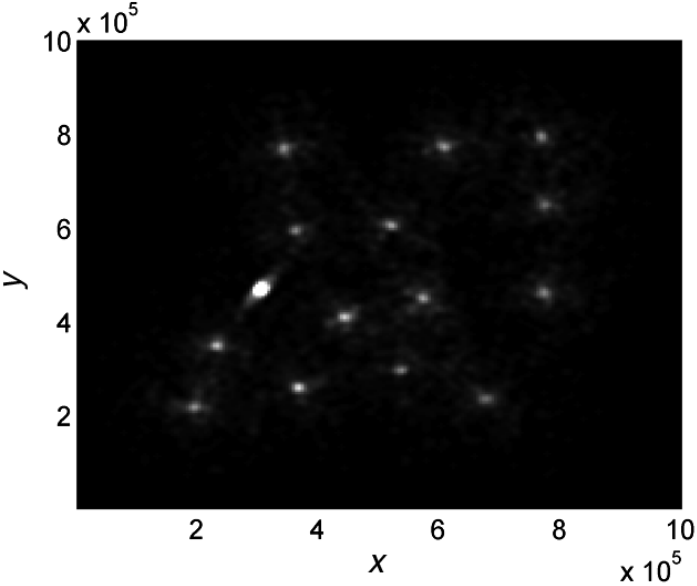
\includegraphics[scale=.15]{4b.png}
    }\\
    \subfigure[直方图上格点的局部密度和最小距离. \label{fig:4c}]{
        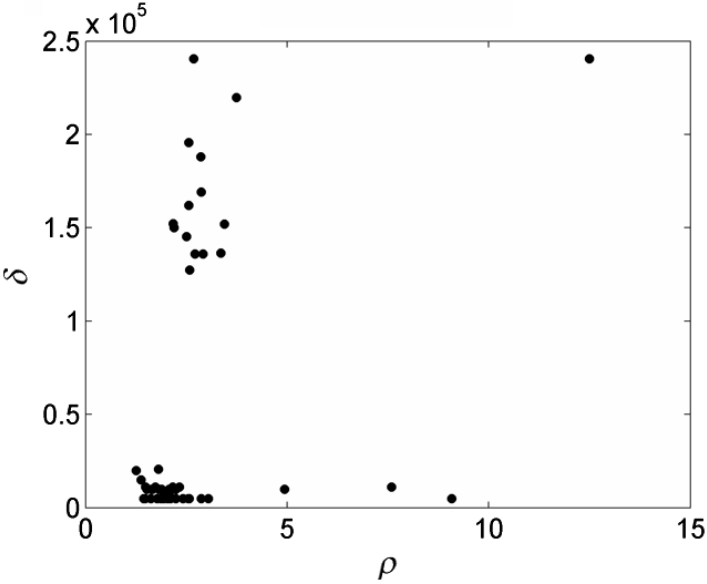
\includegraphics[scale=.15]{4c.png}
    }
    \subfigure[排序后的结果. \label{fig:4d}]{
        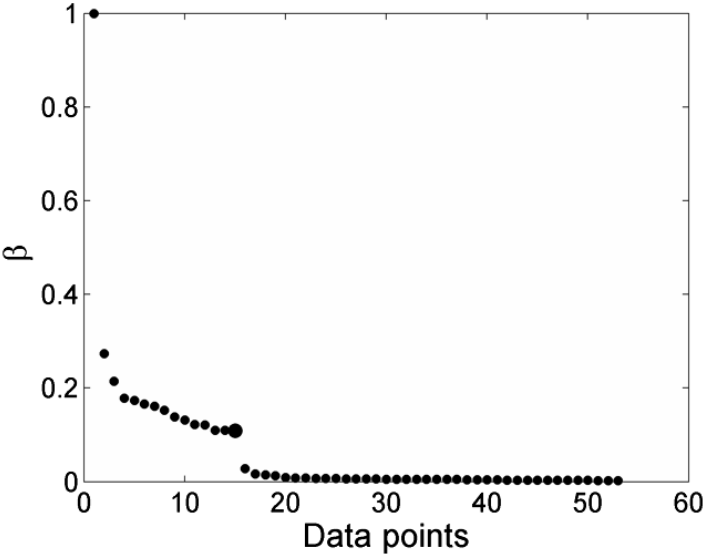
\includegraphics[scale=.15]{4d.png}
    }
    \caption{加速密度聚类算法. 图~\ref{sub@fig:4a} 中的白色圆圈和白色星号分别是密度聚类和加速密度聚类结果的聚类中心. 图~\ref{sub@fig:4d} 中较大的圆点代表聚类中心的决策点. }
\end{figure}
如图~\ref{fig:4a} 所示. 二维的``S"型数据集的在空间分布上具有不同的复杂性. 它有15个预定义的聚类中心. 从图~\ref{fig:4a} 中我们可以看到, 数据点具有非球形的概率分布, 且不同聚类中心所属的概率分布重叠严重. 白色圆圈是密度聚类算法确定的聚类中心. 白色星号是由加速密度聚类算法确定的聚类中心. 可以看到, 加速密度聚类算法计算出的聚类中心与原始密度聚类算法计算出的聚类中心完全吻合. 这个结果表明加速密度聚类可以找到与原始密度聚类相同的极大似然解. 图~\ref{fig:4b} 显示了直方图函数所估计出的局部密度. 二维直方图上的密度峰值点保留了中心信息. 通过将直方图的格点作为一个新的数据集, 大大降低了计算成本, 因为新数据集中的点数量很少. 图~\ref{fig:4c} 给出了每个数据点的局部密度$\rho_i$和新数据集中密度较高的点的最小距离$\sigma_i$. 图~\ref{fig:4d} 是$\beta$的排序结果, 使用的是归并排序(\cite{Satish2010}). 在对$\beta$进行排序后, 选择聚类中心为那些$\beta$相对较大的点. 通常情况下, 聚类中心与其他普通点之间会有一个突变. 利用这一特性, 在排序后的$\beta$上应用梯度算子来检测突变. 在图~\ref{fig:4d} 中, 有突变的点用一个较大的圆点表示. $\beta$值大于或等于这个点的数据点被识别为新数据集的聚类中心. 这些中心给出了原始数据集的真实聚类中心的大致位置. 然后进行聚类中心的更新, 找到真正的中心. 对于一个由$N$个数据点组成的数据集, 加速密度聚类的计算复杂度为$O(1/K(r_M/r_{clu})^4N^2)$, 其中$K$为聚类中心的数量, $r_M$和$r_{clu}$分别为直方图中组距的平均半径和聚类簇的平均半径. 加速密度聚类算法的详细计算复杂度分析见附录~\ref{Appendix:A}. 而密度聚类算法的计算复杂度为$O(N^2)$. 加速密度聚类算法比原密度聚类算法快$K(r_{clu}/r_M)^4$倍. 在`S"型数据集的例子中, 有$5000$个数据点, 在Matlab中编写的新算法在单核CPU上的运行时间为0.3 s, 而原密度聚类算法的运行时间为22 s, 加速后的密度聚类算法速度约原来的为73倍. 

为了更加完整地表示算法的性能, 我们给出了原始数据点的分配结果. 
\begin{figure}[htb]
    \centering
    \subfigure[加速密度聚类算法的分配结果. \label{fig:5a}]{
        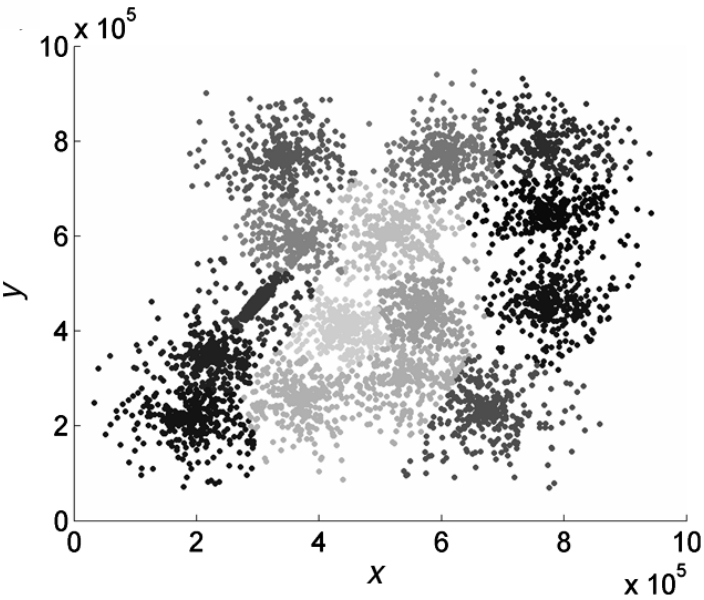
\includegraphics[scale=.15]{5a.png}
    }
    \subfigure[原始密度聚类算法的分配结果. \label{fig:5b}]{
        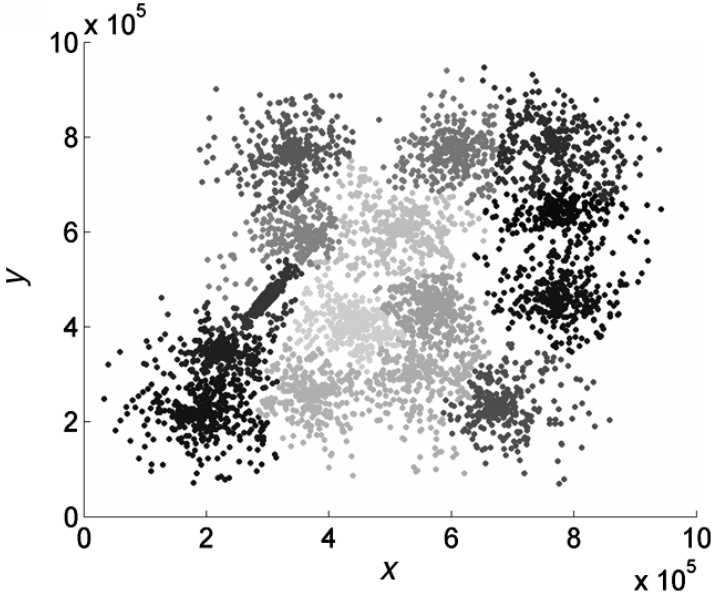
\includegraphics[scale=.15]{5b.png}
    }
    \caption{``S"型数据中数据点的分配结果. 不同灰度表示不同簇. \label{fig:5}}
\end{figure}
图~\ref{fig:5a} 和图~\ref{fig:5a} 分别是我们的算法和原始密度聚类算法的结果. 除了在组的边界处有细微的差异外, 它们的结果十分相似, 这也证明了我们的算法良好性能. 

\subsection{自动速度估计}
通过混合分布模型和加速密度聚类算法的介绍, 我们可以有效地从主要地下构造的同相轴局部斜率中找到映射后的极大似然速度. 主要的反射体通常具有较高的信噪比, 可以很好地被PWD捕获. 通过计算单个CMP道集的映射后的叠加速度$V_{\mathrm{NMO}}(\tau_0)$和零偏距走时$\tau_0$的聚类中心, 我们可以得到了作为结点速度的主反射体的速度. 在所有CMP道集上重复这一过程后, 我们就得到了整个测量的结点速度. 因为假设叠加速度是横向连续的, 所以从相邻CMP道集点映射得到的局部属性可以添加到当前位置作为聚类的输入. 

将自动叠加速度估计扩展到时偏移速度分析上是很直观的. 只需要从堆叠前空间$\{t,h,y\}$映射到时偏移图像空间$\{\tau.x.V_{\mathrm{mig}}\}$(\cite{Fomel2007}), 其中$y$为中点坐标, $\tau$为时偏移双向垂直走时, $V-{\mathrm{mig}}$为时偏移速度, $x$为时偏移图像坐标. 以映射后的局部属性为输入数据, 对每一个成像点道集(CIG)实施加速密度聚, 来提取整个事件的结时偏移速度. 同样的, 对结果进行插值, 建立时偏移速度模型. 

为了将不均匀采样的聚类后的结点速度插入到格网中, 我们可以通过计算一个插值问题: 
\begin{equation}
    \mathbf{G} \mathbf{v}_{\mathbf {grid }}=\mathbf{v}_{\mathbf{k n o t}}
\end{equation}
其中$v_{\mathrm{grid}}$是规则格网上的速度, $v_{\mathrm{knot}}$取不均匀采样上的结点速度, $G$代表插值算子, 在我们的例子中是立方B-splines插值. 由于我们的目标是建立平稳的时域速度模型, 所以在最小二乘目标函数中加入了一个正则化项$\epsilon$: 
\begin{equation}
\left\|\mathbf{G} \mathbf{v}_{\mathbf {grid }}-\mathbf{v}_{\mathbf{k n o t}}\right\|_{2}^{2}+\varepsilon^{2}\left\|\mathbf{L} \mathbf{v}_{\mathbf{g r i d}}\right\|_{2}^{2}
\end{equation}
其中L代表一个粗化算子(如Laplacian算子). 目标函数的最小化结果为: 
\begin{equation}
    \mathbf{v}_{\mathbf{g r i d}}=\left(\mathbf{G}^{T} \mathbf{G}+\varepsilon^{2} \mathbf{L}^{T} \mathbf{L}\right)^{-1} \mathbf{G}^{T} \mathbf{v}_{\mathbf{k n o t}}
\end{equation}

通过上述公式, 我们建立了规则格网上的速度模型. 这个时域速度模型可以进一步用于时域成像任务. 
